%
% The first command in your LaTeX source must be the \documentclass command.
\documentclass[sigconf]{acmart}
\usepackage{tabularx}
\usepackage{multirow}
\usepackage{csvsimple}
\usepackage{mhchem}
\usepackage{graphicx}
\usepackage{subcaption}
\usepackage{mwe}
\usepackage{float}
\usepackage{placeins}
\usepackage{amsfonts}
\usepackage{booktabs}
\usepackage{siunitx}
\settopmatter{printacmref=false}
%
% defining the \BibTeX command - from Oren Patashnik's original BibTeX documentation.
\def\BibTeX{{\rm B\kern-.05em{\sc i\kern-.025em b}\kern-.08emT\kern-.1667em\lower.7ex\hbox{E}\kern-.125emX}}
    
% Rights management information. 
% This information is sent to you when you complete the rights form.
% These commands have SAMPLE values in them; it is your responsibility as an author to replace
% the commands and values with those provided to you when you complete the rights form.
%
% These commands are for a PROCEEDINGS abstract or paper.
\copyrightyear{2018}
\acmYear{2018}
\setcopyright{acmlicensed}
\acmConference[e-Energy '19]{e-Energy '19: The Tenth International Conference on Future Energy Systems}{June 25--28, 2019}{Phoenix, AZ}
\acmPrice{15.00}
\acmDOI{10.1145/1122445.1122456}
\acmISBN{978-1-4503-9999-9/18/06}


%
% These commands are for a JOURNAL article.
%\setcopyright{acmcopyright}
%\acmJournal{TOG}
%\acmYear{2018}\acmVolume{37}\acmNumber{4}\acmArticle{111}\acmMonth{8}
%\acmDOI{10.1145/1122445.1122456}

%
% Submission ID. 
% Use this when submitting an article to a sponsored event. You'll receive a unique submission ID from the organizers
% of the event, and this ID should be used as the parameter to this command.
%\acmSubmissionID{123-A56-BU3}

%
% The majority of ACM publications use numbered citations and references. If you are preparing content for an event
% sponsored by ACM SIGGRAPH, you must use the "author year" style of citations and references. Uncommenting
% the next command will enable that style.
%\citestyle{acmauthoryear}

%
% end of the preamble, start of the body of the document source.

\begin{document}

%
% The "title" command has an optional parameter, allowing the author to define a "short title" to be used in page headers.

%\title[Modelling Carbon Tax]{Modelling Carbon Tax in the UK Electricity Market using Agent-Based Models}
\title{Modelling Carbon Tax in the UK Electricity Market using an Agent-Based Model}


%
% The "author" command and its associated commands are used to define the authors and their affiliations.
% Of note is the shared affiliation of the first two authors, and the "authornote" and "authornotemark" commands
% used to denote shared contribution to the research.

%\author{Anonymized}

\author{Alexander Kell}
\affiliation{%
  \department{School of Computing}
  \institution{Newcastle University}
  \city{Newcastle upon Tyne}
  \country{UK}
}
\email{a.kell2@newcastle.ac.uk}

\author{Matthew Forshaw}
\affiliation{%
  \department{School of Computing}
  \institution{Newcastle University}
  \city{Newcastle upon Tyne}
  \country{UK}
}
\email{matthew.forshaw@newcastle.ac.uk}

\author{A. Stephen McGough}
\affiliation{%
  \department{School of Computing}
  \institution{Newcastle University}
  \city{Newcastle upon Tyne}
  \country{UK}
}
\email{stephen.mcgough@newcastle.ac.uk}
 
%
% By default, the full list of authors will be used in the page headers. Often, this list is too long, and will overlap
% other information printed in the page headers. This command allows the author to define a more concise list
% of authors' names for this purpose.


%\renewcommand{\shortauthors}{Kell et al.}

%
% The abstract is a short summary of the work to be presented in the article.
\begin{abstract}

Impacts on natural and human systems have already been observed due to anthropogenic greenhouse gas emissions \cite{Masson-Delmotte2018}. To reduce these emissions, a transition to a low-carbon economy is required. Carbon taxes can be used as a tool for pricing in the negative externalities of pollution and enabling a more rapid transition to a low-carbon economy.

This paper proposes the use of agent-based models to simulate an electricity market based in the United Kingdom. We vary carbon tax to observe the effects on investment up until 2050. We find that a carbon tax of \textsterling70 per tonne of \ce{CO2} is sufficient in driving investment to an almost 100\% renewable energy supply. A less aggressive option, however, of setting a carbon tax at \textsterling20 would lead to a 50\% low-carbon, 50\% traditional generation energy mix.


\end{abstract}

%
% The code below is generated by the tool at http://dl.acm.org/ccs.cfm.
% Please copy and paste the code instead of the example below.
%

%
% Keywords. The author(s) should pick words that accurately describe the work being
% presented. Separate the keywords with commas.

% \keywords{agent-based modelling, simulation, energy market simulation, energy models, policy}

%
% A "teaser" image appears between the author and affiliation information and the body 
% of the document, and typically spans the page. 

%
% This command processes the author and affiliation and title information and builds
% the first part of the formatted document.
\maketitle


\section{Introduction}

Governmental policy is a tool that can be used to aid in the transition to a low-carbon economy to prevent the worst effects of climate change. Options include a tax on all carbon emissions or subsidies in low-carbon technologies. In this paper, we vary carbon taxes to assess the long-term impacts on investment in the electricity market. We used a general agent-based model simulation made for wholesale electricity markets, created by us. 


Simulation is a technique to create a physical system in a virtual world.  In this context a model is defined as a set of mathematical formulas and algorithms which are designed to mimic real life \cite{Forshaw2016}. Simulation allows practitioners to rapidly prototype high risk ideas in this virtual model and assess their outcome before implementation in the real world.

The electricity market in many western democracies consists of multiple heterogenous actors acting for their own best interest \cite{Most2010}. Agent-based modelling is a technique which allows for the simulation of these heterogenous actors with different risk profiles, profit requirements and preferences. A number of agent-based models have been used to model the impact of carbon tax on long term investments \cite{Tang2015, Chen2014, Chappin2017}. ABMs have been utilised in this field to address phenomena such as market power \cite{Ringler2016a}.

We model the realisation of the wholesale electricity market in the United Kingdom and adjust carbon tax in our agent-based model to see the effect of long-term investment. Whilst we have modelled the United Kingdom, it would be possible to model for any country with different parameters. We posit that decisions made today can have complex long-term consequences, the process of which can be observed through simulation.



This paper details our model and different carbon scenarios. Section \ref{Model} details the model, assumptions made and parameters. Section \ref{Scenario Testing} presents our results. We conclude our work in Section \ref{Conclusion} and explore possible routes forward .







\section{Model Architecture} \label{Model}

\begin{figure}
	\centering
	\includegraphics[width=0.97\linewidth]{figures/System_overview}
	\caption{System overview of agent-based market model.}
	\label{fig:systemoverview}
\end{figure}

\begin{figure*}[h]
	\centering
	\begin{subfigure}[b]{0.33\textwidth}
		\centering
		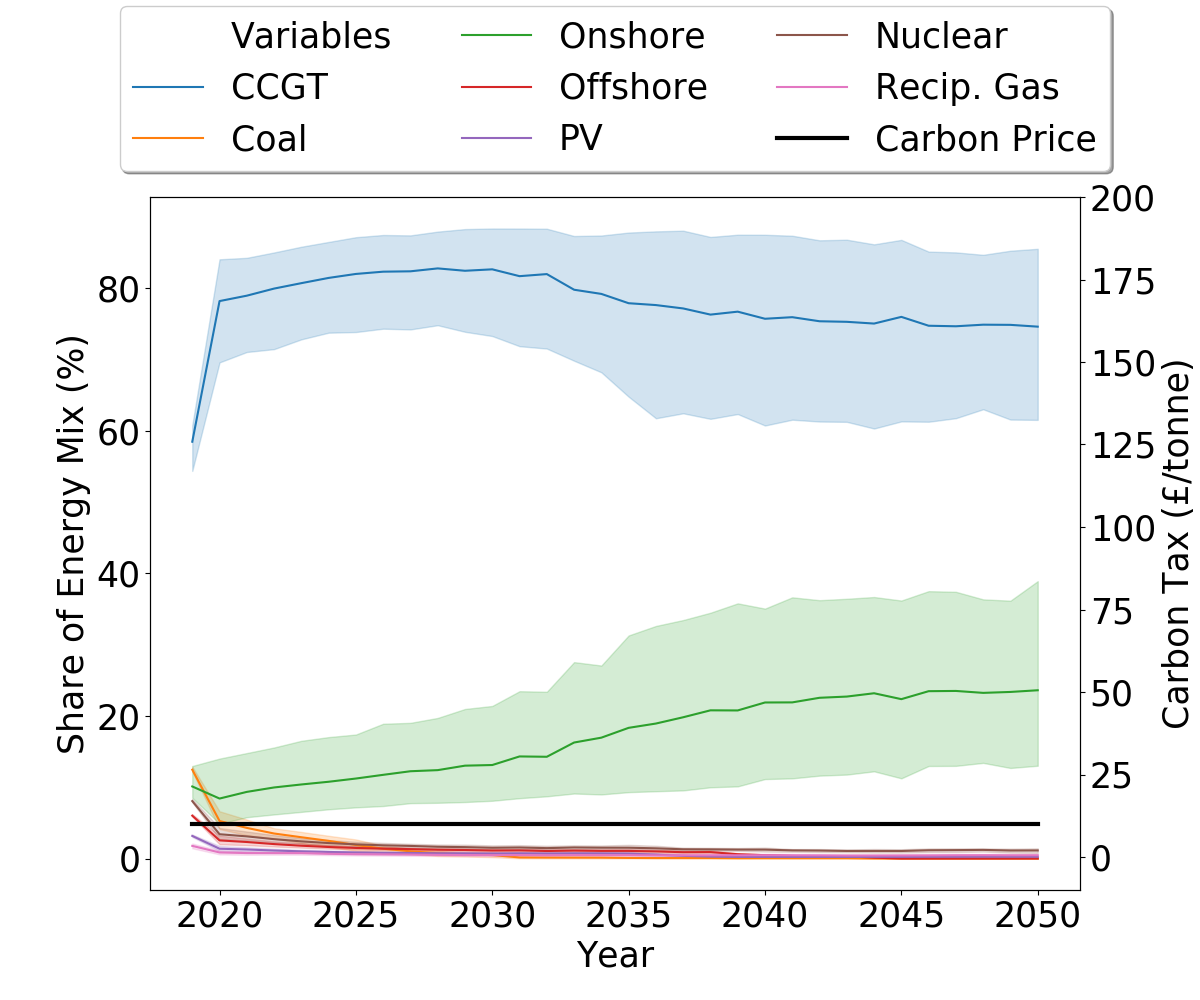
\includegraphics[width=\textwidth]{figures/scenarios/demand099-carbon10-datetime.png}
		\caption[Network2]%
		{\small \textsterling10 carbon tax.}
		\label{fig:demand99carbon10}
	\end{subfigure}
	\hfill
	\begin{subfigure}[b]{0.33\textwidth}  
		\centering 
		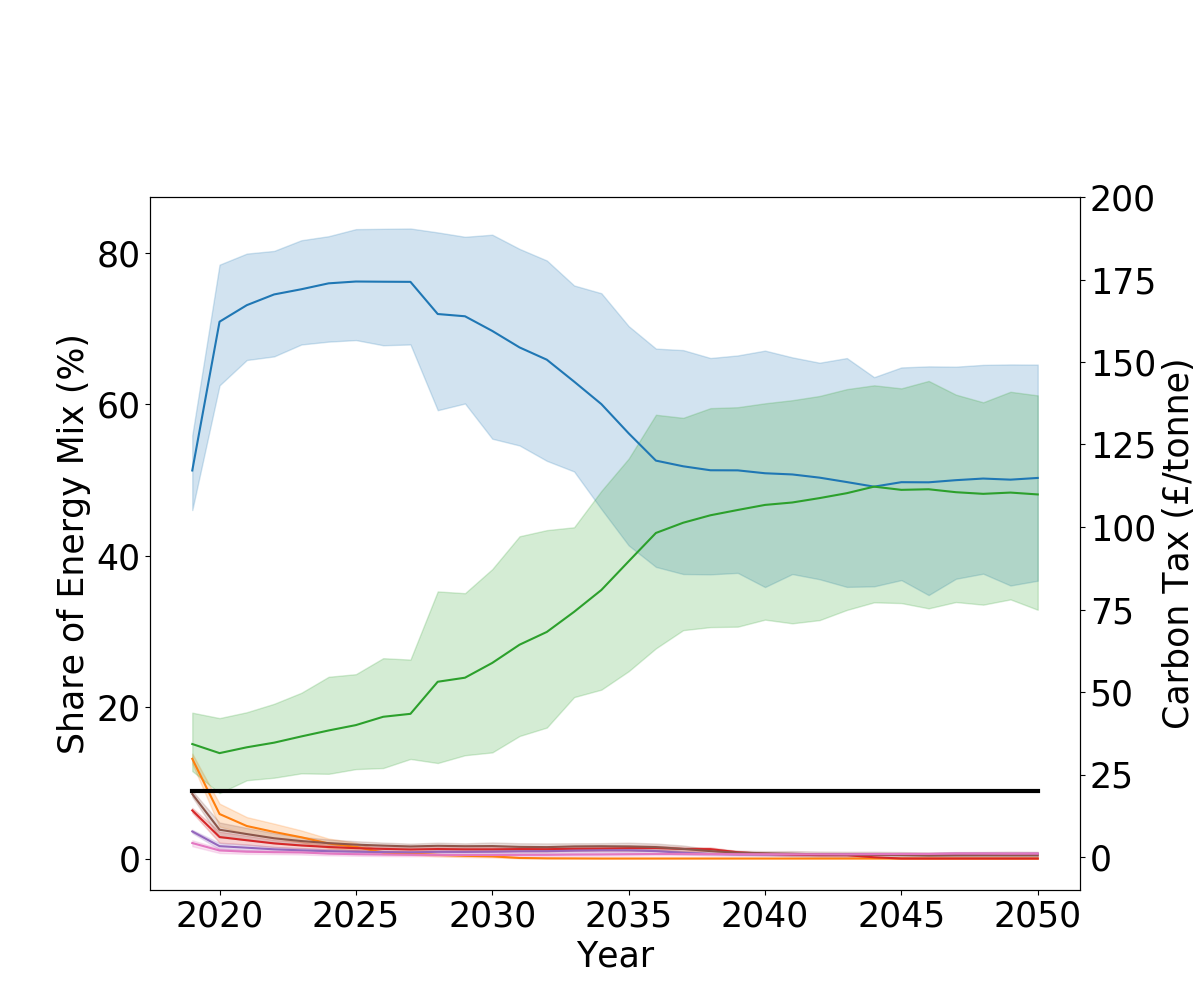
\includegraphics[width=\textwidth]{figures/scenarios/demand099-carbon20-datetime.png}
		\caption[]%
		{\textsterling20 carbon tax.}
		\label{fig:demand99carbon20}
	\end{subfigure}
	\begin{subfigure}[b]{0.33\textwidth}
		\centering
		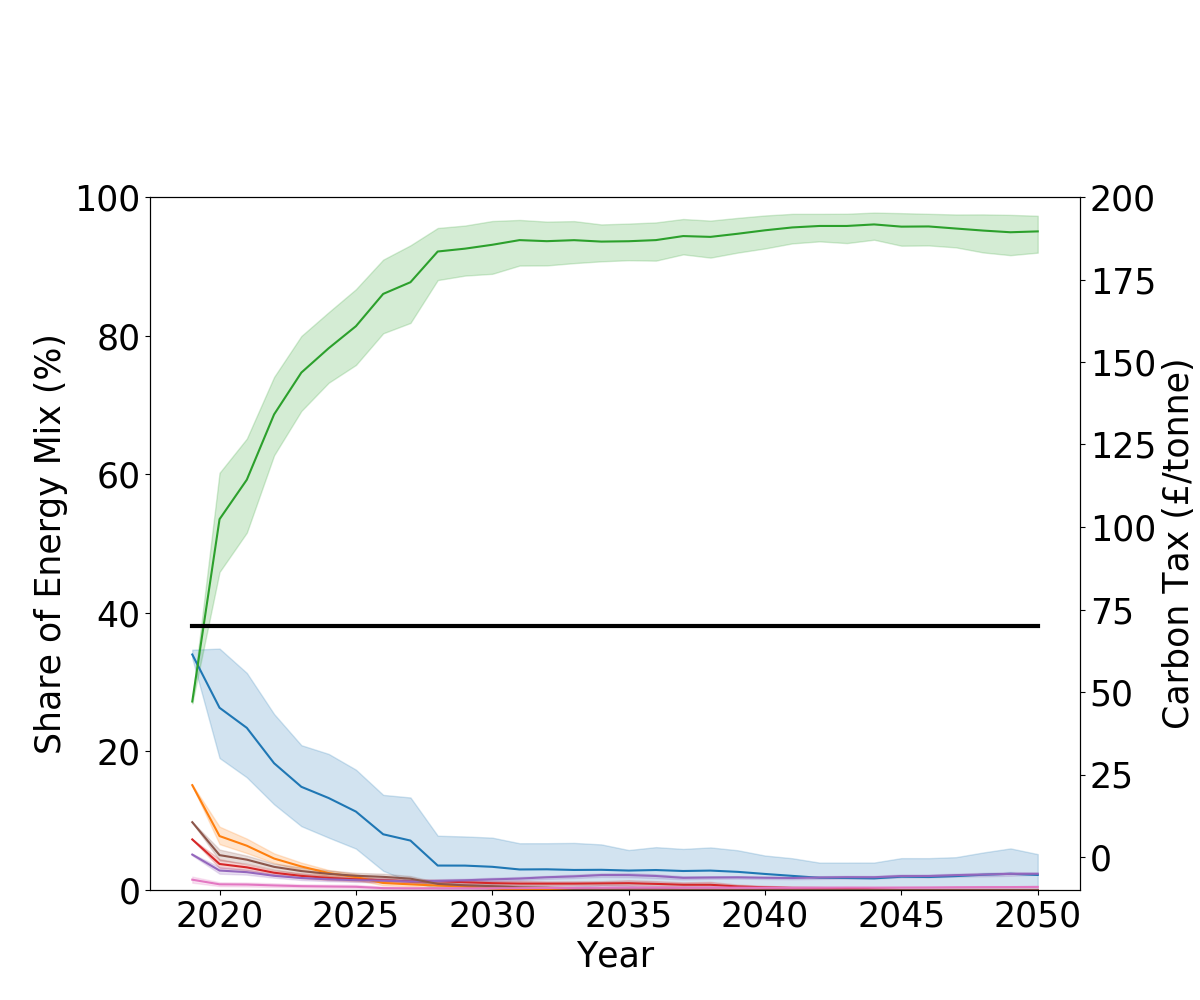
\includegraphics[width=\textwidth]{figures/scenarios/demand099-carbon70-datetime.png}
		\caption[Network2]%
		{\small \textsterling70 carbon tax.}
		\label{fig:demand99carbon10}
	\end{subfigure}
	\vskip\baselineskip
\end{figure*}


The agent-based model is made up of five significant parts: the agents which are the generation companies (GenCos) and demand agents; power plants and a market operator which controls the spot market. How these parts interact are displayed in figure \ref{fig:systemoverview} with the relevant data sources.

We initialise the United Kingdom with every single power plant in operation in the year 2018, owned by their respective generation companies . Individual historical power plant costs are estimated from levelized cost of electricity (LCOE) \cite{Dale2013} calculations \cite{IEA2015,IRENA2018}, whereas future power plants are taken from the department of business and industrial strategy \cite{Department2016}. The variable operation and maintenance cost was defined stochastically to model the changing costs per project. A uniform distribution was chosen to provide sufficient variance between projects.

The demand agent is modelled as a single aggregated demand, split up into 20 segments of a load duration curve (LDC), enabling us to increase speed of computation whilst maintaining accuracy. A LDC is defined as the load within a year, ordered in order of magnitude. 

We model the influence of outages using availability data for gas, coal, photovoltaic, offshore and onshore power generators \cite{Ltd2016, Hunt2015, carroll-j}. Historical availabilities are modelled for older gas, coal and hydro power plants \cite{AlbertaSystemElectricOperator2016}. Capacity factors were taken as an average of the UK for solar and wind \cite{Pfenninger2016, Staffell2016}. Where capacity factors is defined as the ratio of electrical output over a given time period over the maximum possible electrical energy output. 

The generation companies make electricity bids each year for each of their power plants. The market operator then matches demand with supply in order of price, also known as merit-order dispatch. We model a uniform pricing market, where each of the companies are paid the highest accepted bid.

GenCos have the ability to invest every year in new power plants based on the expected net present value (NPV) of each power plant type. NPV is a summation of the present value of a series of present and future cash flow. The NPV calculation is dependent on a stochastic representation of GenCos predictions of fuel, carbon and electricity price and demand.

Each GenCo has a separate weighted average cost of capital (WACC), which is the rate that a company is expected to pay on average for its stock and debt, this is used as the discount rate in the NPV calculation \cite{KincheloeStephenC1990TWAC}. The WACC is modelled as a stochastic variable, with a Gaussian distribution and a $\pm3\%$ standard deviation, with values of 5.9\% for non-nuclear power plants, and 10\% for nuclear power plants \cite{KPMG2017, Paper2012}. 

The model took yearly time-steps to limit the impact on computation time, however, to model the intermittency of renewable generation, we correlated demand with the respective capacity factor, enabling for example, solar and wind to only contribute a certain capacity to their load curve.

Stochasticity of fuel price within a year was also modelled, to take into account difference in hedging strategies and chance. An ARIMA model \cite{ARIMA} was fit to historic coal and natural gas prices.






\section{Results}\label{Scenario Testing}

We experimented with the following levels of carbon tax: \textsterling10 (\$13), \textsterling20 (\$26) and \textsterling70 (\$90) with demand decreasing 1\% per year. We chose this due to the increasing efficiency of homes, industy and technology, and due to the recent trend in the UK. We run each scenario 8 times each to capture the stochastic nature of the process. Via the observation of the emergent investment behaviour until 2050, an understanding of how real life investors may behave emerges.


Figure \ref{fig:demand99carbon10} shows that with a carbon tax of \textsterling10, whilst renewable technology does grow, gas power plants provide the majority of supply in each year. However, at a level of \textsterling20 the increase in wind turbines is enough to match gas turbines. A carbon tax of \textsterling70, however, shows a near 100\% uptake of wind turbines.

It is infeasible for the power supply to be provided solely by wind turbines today. This overestimation, however, is due to the low time granularity of the model \cite{Collins2017}. This scenario therefore assumes perfect storage capabilities.






%\FloatBarrier








%\begin{figure}[h]
%	\begin{center}
%		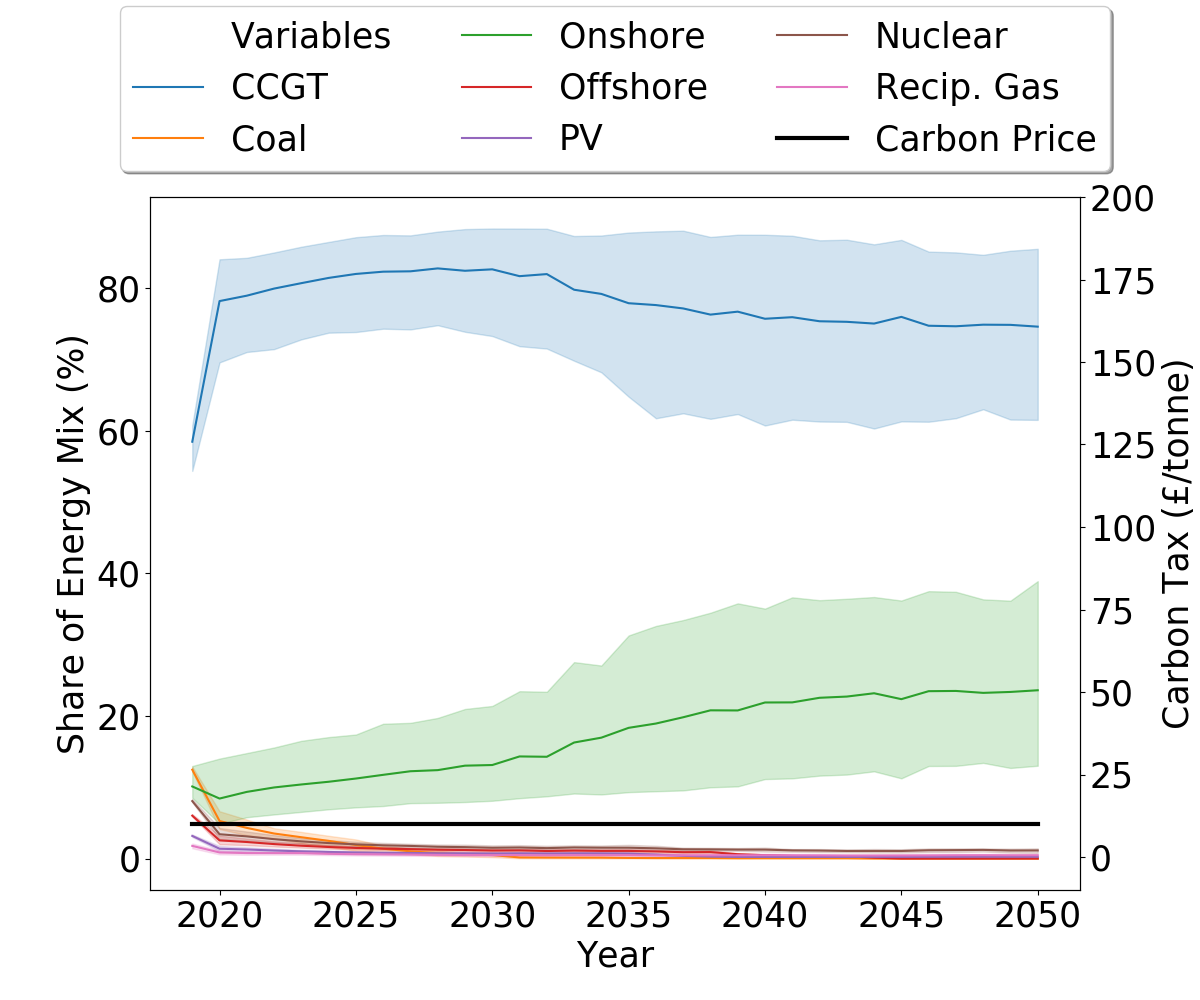
\includegraphics[width=0.5\textwidth]{figures/scenarios/demand099-carbon10-datetime.png}
%		\caption{Demand decreasing by 1\% per year and a carbon tax of \textsterling10}
%		\label{fig:demand99carbon10}
%	\end{center}
%\end{figure}
%
%\begin{figure}[h]
%	\begin{center}
%		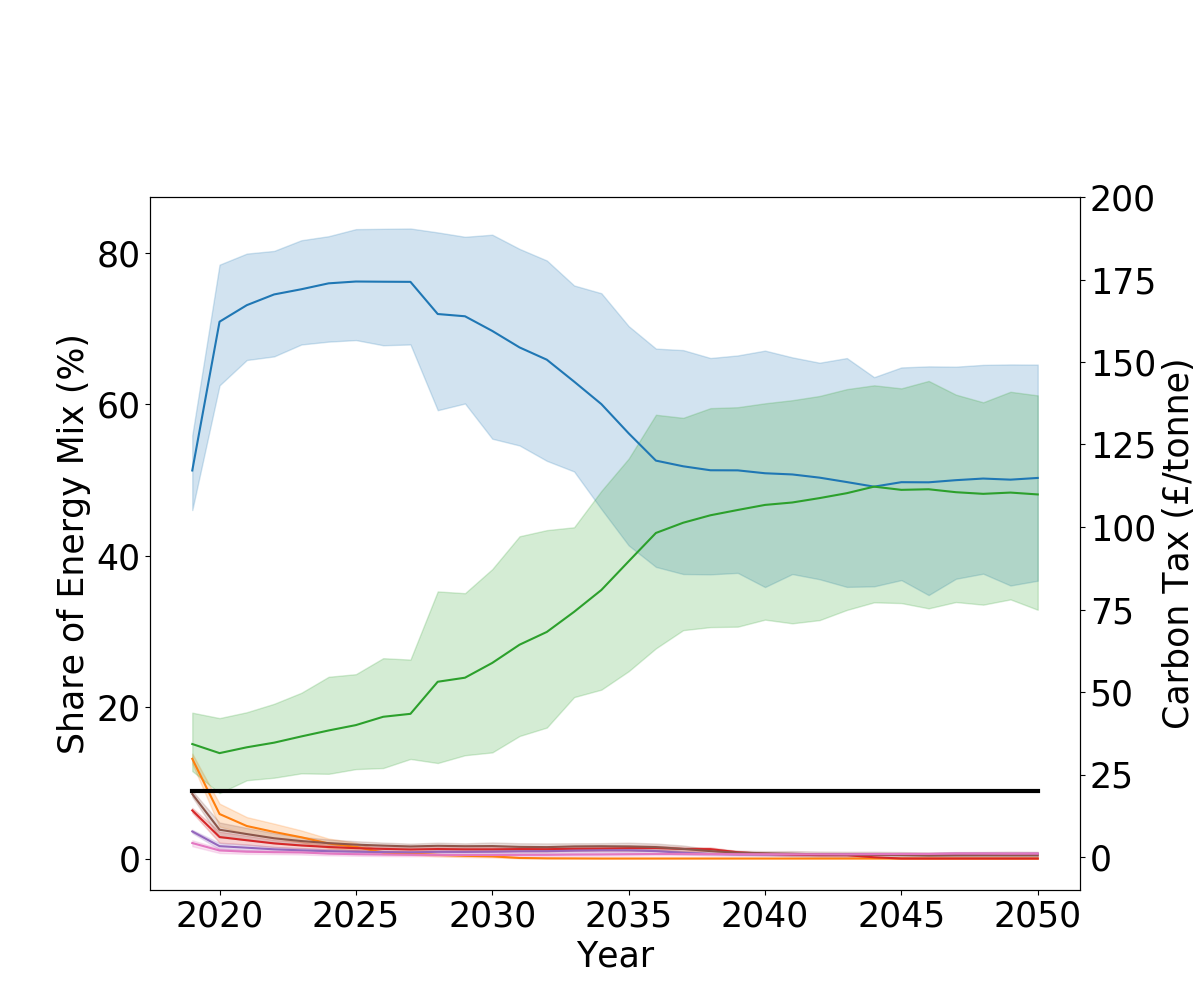
\includegraphics[width=0.5\textwidth]{figures/scenarios/demand099-carbon20-datetime.png}
%		\caption{Demand decreasing by 1\% per year and a carbon tax of \textsterling20}
%		\label{fig:demand99carbon10}
%	\end{center}
%\end{figure}
%
%
%
%\begin{figure}[h]
%	\begin{center}
%		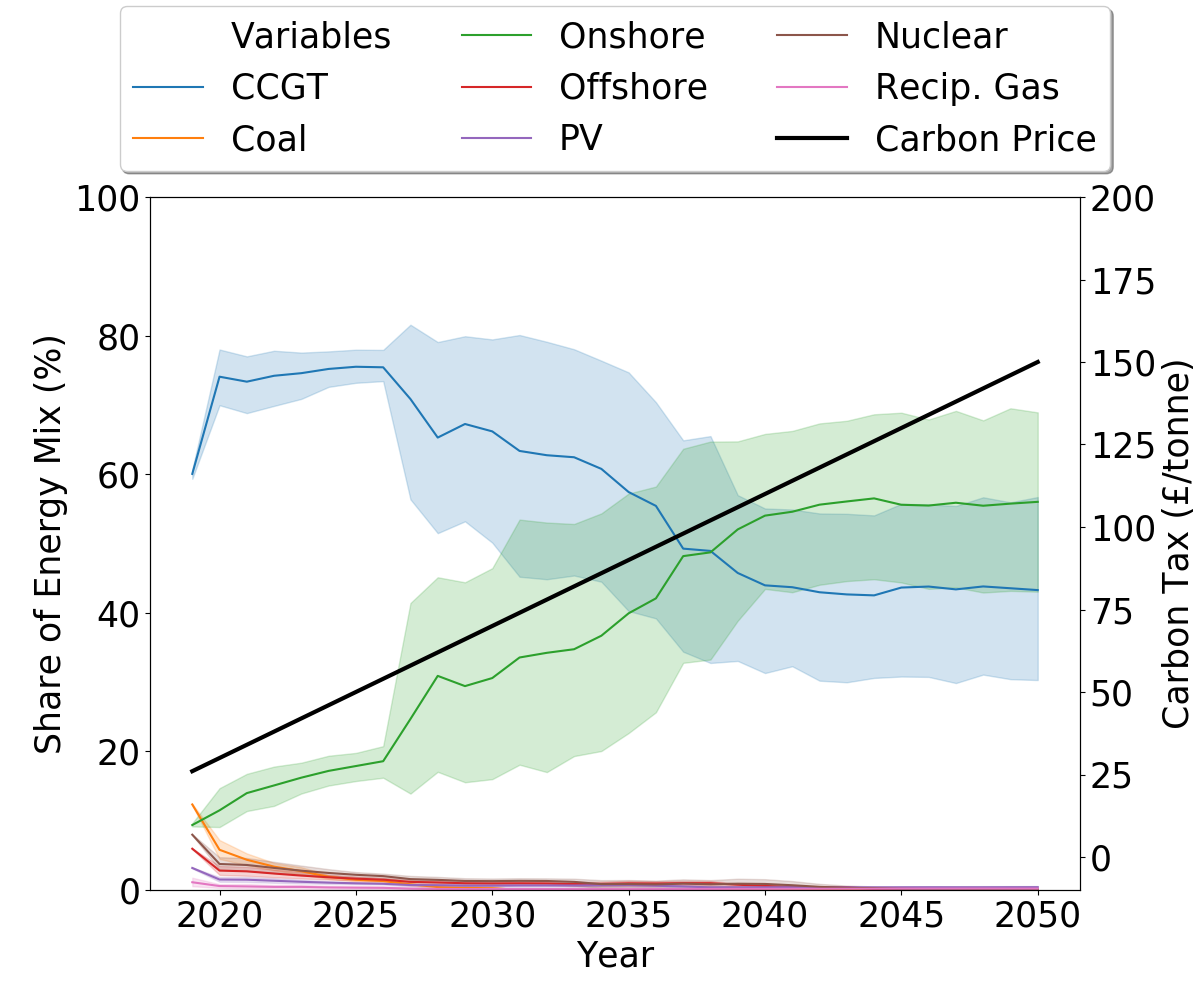
\includegraphics[width=0.5\textwidth]{figures/scenarios/demand099-carbon18-datetime.png}
%		\caption{Demand decreasing by 1\% per year and a carbon tax of \textsterling20}
%		\label{fig:demand99carbon10}
%	\end{center}
%\end{figure}
%
%
%
%\begin{figure}[h]
%	\begin{center}
%		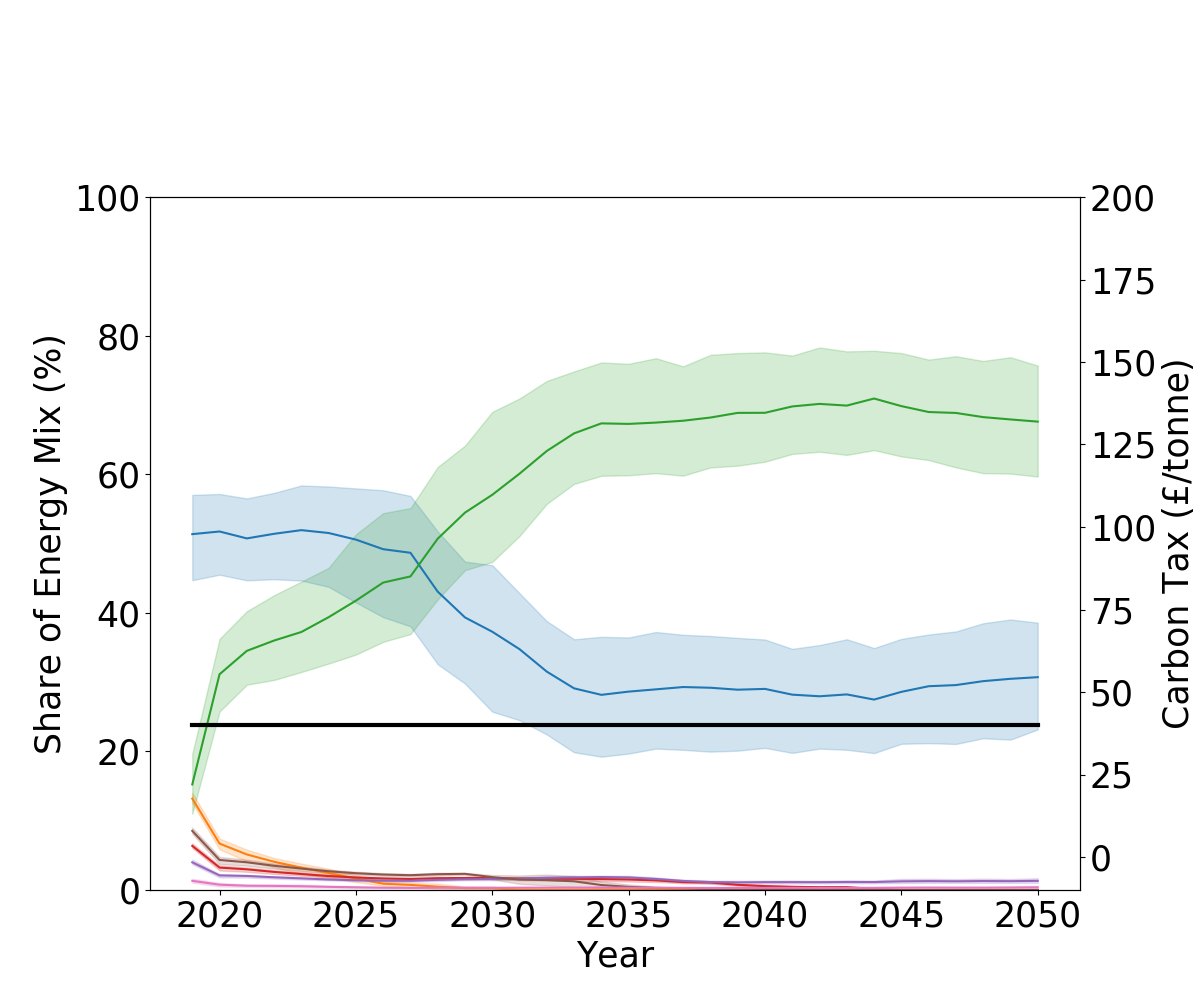
\includegraphics[width=0.5\textwidth]{figures/scenarios/demand099-carbon40-datetime.png}
%		\caption{Demand decreasing by 1\% per year and a carbon tax of \textsterling20}
%		\label{fig:demand99carbon10}
%	\end{center}
%\end{figure}











%\begin{itemize}
%	\item Effect of different carbon tax on investments made.
%	\item Effects of different demand scenarios. (High peaks, high growth, high reduction in demand)
%	\item Effects of high fuel prices.
%	\item Different costs of capital (eg. Borrowing for Nuclear of interest rate to equal 2\% at government bonds rate, as opposed to 10\% for private companies.)
%	\item Different learning rates for renewable costs.
%	\item The effect of long term carbon tax policy (eg. Carbon price known for next 25 years) vs short term changes in carbon tax.
%\end{itemize}




\section{Conclusions}\label{Conclusion}

Agent-based models provide a method of simulating investor behaviour in an electricity market. Using this technique, we were able to observe the emergent investor behaviour. 

We observed that an increase in carbon tax had a significant impact on investment. These findings enable policy makers to better understand the impact that their decisions may have. For a high uptake of renewable energy technology, rapid results can be seen after 10 years with a carbon tax of \textsterling70.

Agent-based models open up the possibility of testing differing investor behaviours through techniques such as reinforcement learning. This can be extended to incorporate collusion which can have an impact in liberalized electricity markets\cite{Benjamin2016}.

We propose the integration of a higher temporal and spatial resolution to model the utility of batteries, distributed generation and scarceness in renewable resources such as wind and solar.


\FloatBarrier




%
% The acknowledgments section is defined using the "acks" environment (and NOT an unnumbered section). This ensures
% the proper identification of the section in the article metadata, and the consistent spelling of the heading.


\begin{acks}
This work was supported by the Engineering and Physical Sciences Research Council, Centre for Doctoral Training in Cloud Computing for Big Data [grant number EP/L015358/1].
\end{acks}

\clearpage

%
% The next two lines define the bibliography style to be used, and the bibliography file.
\bibliographystyle{ACM-Reference-Format}
\bibliography{library,custombibtex}

% 
% If your work has an appendix, this is the place to put it.
%\appendix
%
%
%\section{Research Methods}
%\input{appendix}


\end{document}
